The model of the distribution of decay time and decay angles in the \BstoJpsiKK{} decay is fitted to the data from reconstructed and
selected $\Bs$ and $\Bsbar$ candidates, after background subtraction. Statistical uncertainties in the resulting parameter estimates are
evaluated with the shape of the likelihood function. Systematic uncertainties are estimated by repeating the fit with variations of the
model or the data.

Results are presented for three different parameterizations of CP violation. Different assumptions are made, based on the facts that the
\BstoJpsiKK{} decay is dominated by a tree-level amplitude and that CP violation in mixing is small, as discussed in
Section~\ref{subsec:intro_Jpsiphi_decay}. If contributions from additional amplitudes are small, CP violation is induced by the \BsBsbar{}
mixing process and does not depend on the intermediate state. Also CP violation in decay will be small in this case.

The first parameterization is most general and includes different parameters $\phisi$ and $\Csi$ or the intermediate states
$i\in\{\text{0}, \parallel, \perp, \text{S}\}$. See Section~\ref{sec:pheno_equations} for a description of the actual parameters that
are used. The second parameterization is more restrictive and assumes no CP-violation differences between the intermediate states. For the
third parameterization the additional assumptions of no CP violation in mixing and no CP-violation in decay are made. The following
parameters describe CP violation for these three cases:
\begin{enumerate}
  \item $\phisav,\Delphispara,\Delphisperpp,\DelphisS
         \quad\text{and}\quad\Csav,\DelCspara,\DelCsperp,\CsavS$
  \item $\phisi[\text{0}]=\phisi[\parallel]=\phisi[\perp]=\phisi[\text{S}]\equiv\phis
         \quad\text{and}\quad\lamsiAbs[\text{0}]=\lamsiAbs[\parallel]=\lamsiAbs[\perp]=\lamsiAbs[\text{S}]\equiv\lamsAbs$
  \item $\phisi[\text{0}]=\phisi[\parallel]=\phisi[\perp]=\phisi[\text{S}]\equiv\phis
         \quad\text{and}\quad\lamsiAbs[\text{0}]=\lamsiAbs[\parallel]=\lamsiAbs[\perp]=\lamsiAbs[\text{S}]\equiv1$
\end{enumerate}

Figures~\ref{fig:timeProjections} and \ref{fig:angleProjections} show the background-subtracted distributions of decays in time and angles
and the corresponding one-dimensional PDF projections for the $\phis$/$\lamsAbs$ model. The decay-time distribution is shown in both the
full selected range of [0.3, 14]~ps on a logarithmic vertical scale (Figure~\ref{fig:timeProjections_log}) and in a reduced range of [0.3,
5]~ps on a linear vertical scale (Figure~\ref{fig:timeProjections_lin}).
\begin{figure}[htb]
  \centering
  \begin{subfigure}{0.49\textwidth}
    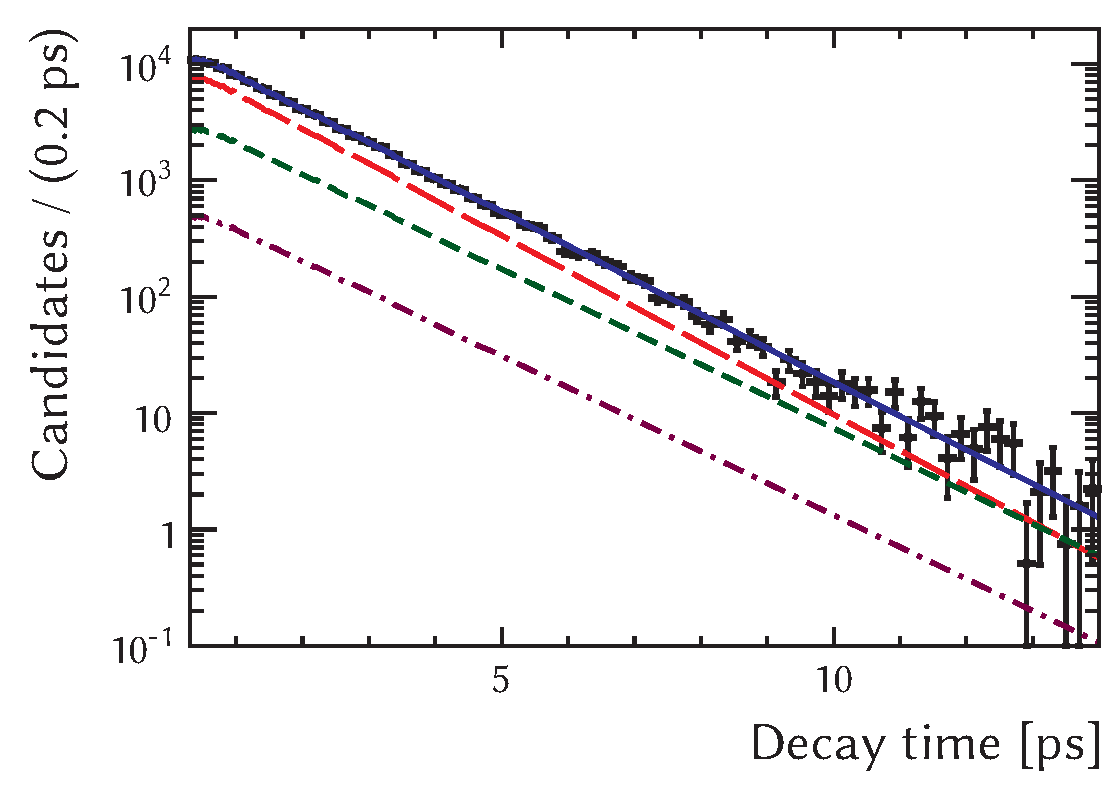
\includegraphics[width=\textwidth]{graphics/results/timeLog}
    \caption{}
    \label{fig:timeProjections_log}
  \end{subfigure}
  \hfill%
  \begin{subfigure}{0.49\textwidth}
    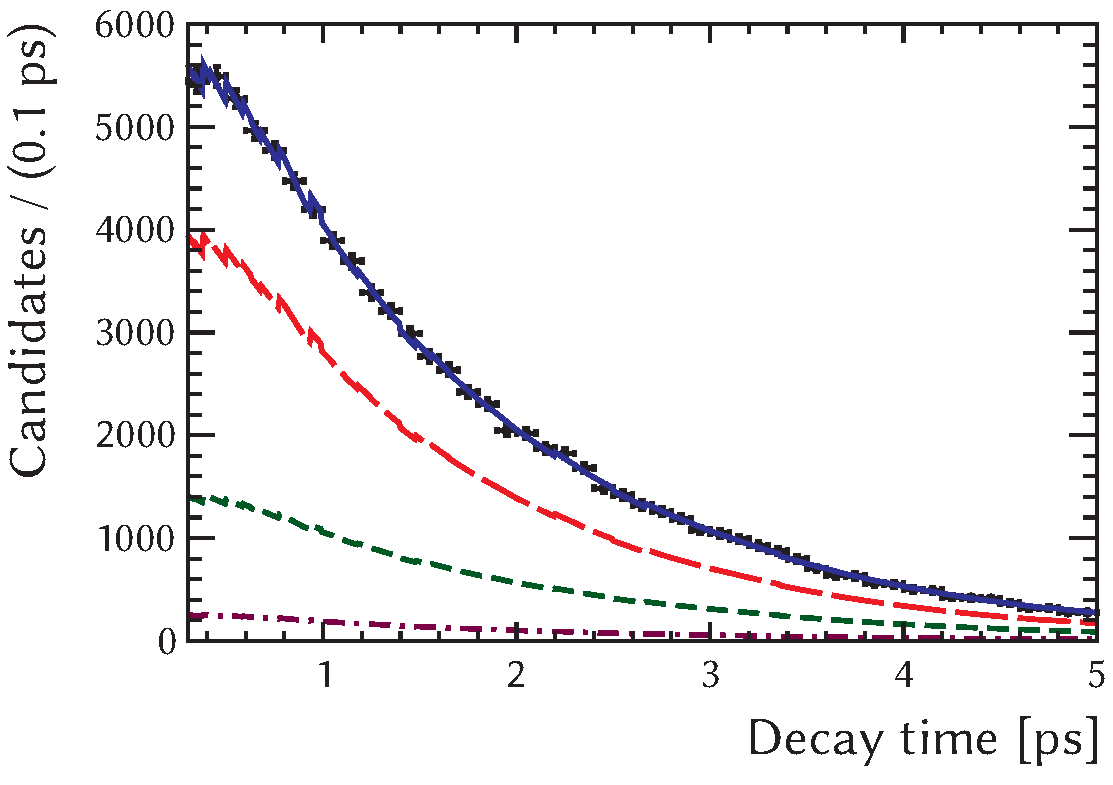
\includegraphics[width=\textwidth]{graphics/results/timeLin}
    \caption{}
    \label{fig:timeProjections_lin}
  \end{subfigure}

  \caption{Background-subtracted distribution of decays in decay time (data points)
           and the corresponding one-dimensional projection of the PDF (blue line).
           Figure~(a) shows the distribution in the full range between 0.3 and 14\unitsp{}ps
           on a logarithmic vertical scale, while Figure~(b) shows the distribution between 0.3 and 5\unitsp{}ps
           on a linear vertical scale.
           Additional PDF projections are shown for the CP-even (long-dashed, red line) and CP-odd (short-dashed, green line)
           components of \BstoJpsiphi{} and for the S-wave (dashed-dotted, magenta line).}
  \label{fig:timeProjections}
\end{figure}
%
\begin{figure}[htbp]
  \centering
  \begin{subfigure}{0.49\textwidth}
    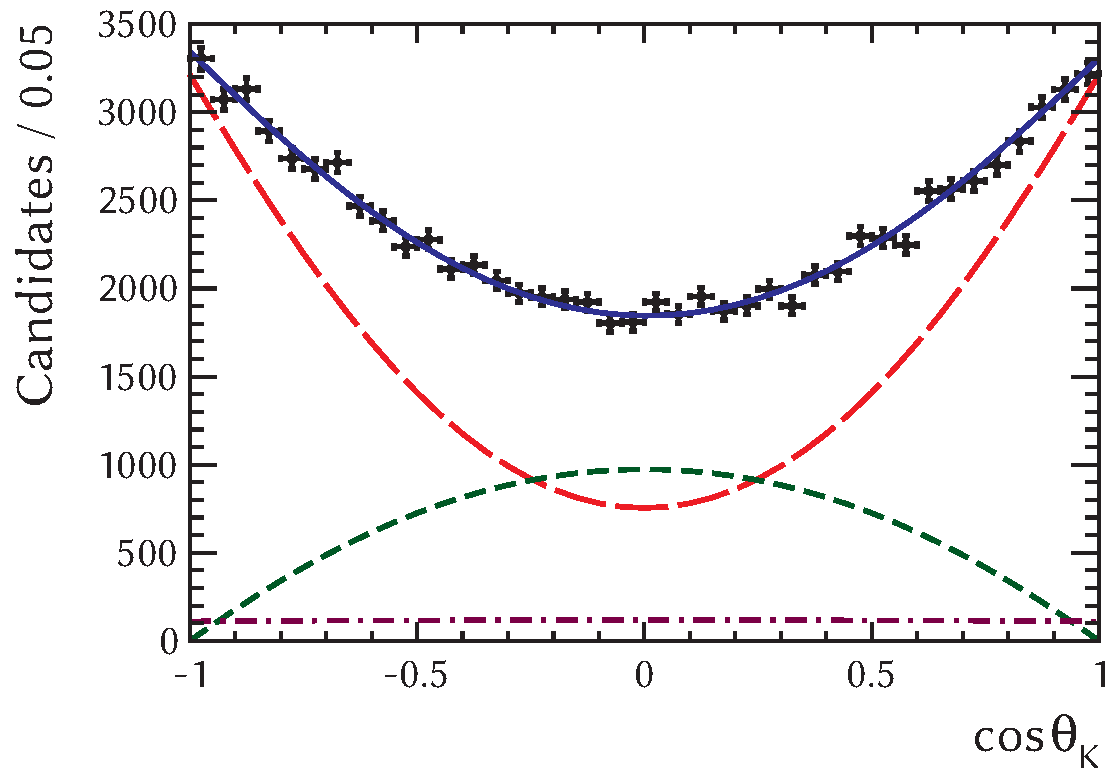
\includegraphics[width=\textwidth]{graphics/results/ctk}
    \caption{}
  \end{subfigure}
  \hfill%
  \begin{subfigure}{0.49\textwidth}
    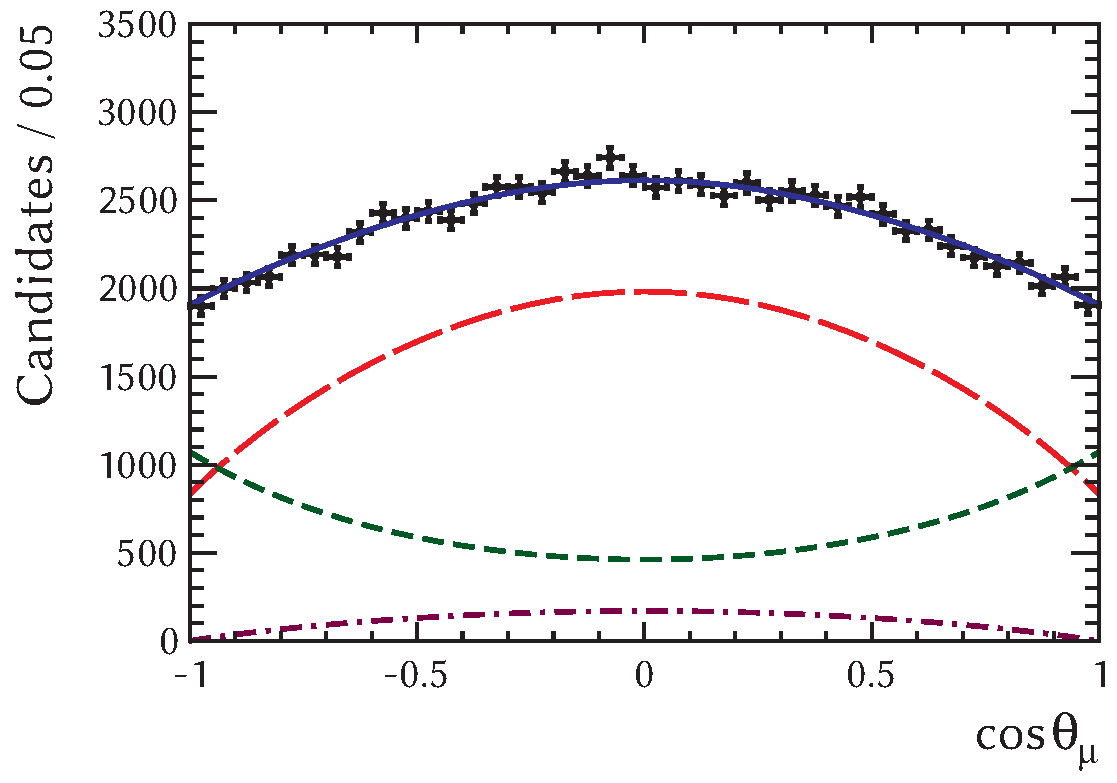
\includegraphics[width=\textwidth]{graphics/results/ctl}
    \caption{}
  \end{subfigure}

  \vspace*{0.02\textwidth}
  \begin{subfigure}{0.49\textwidth}
    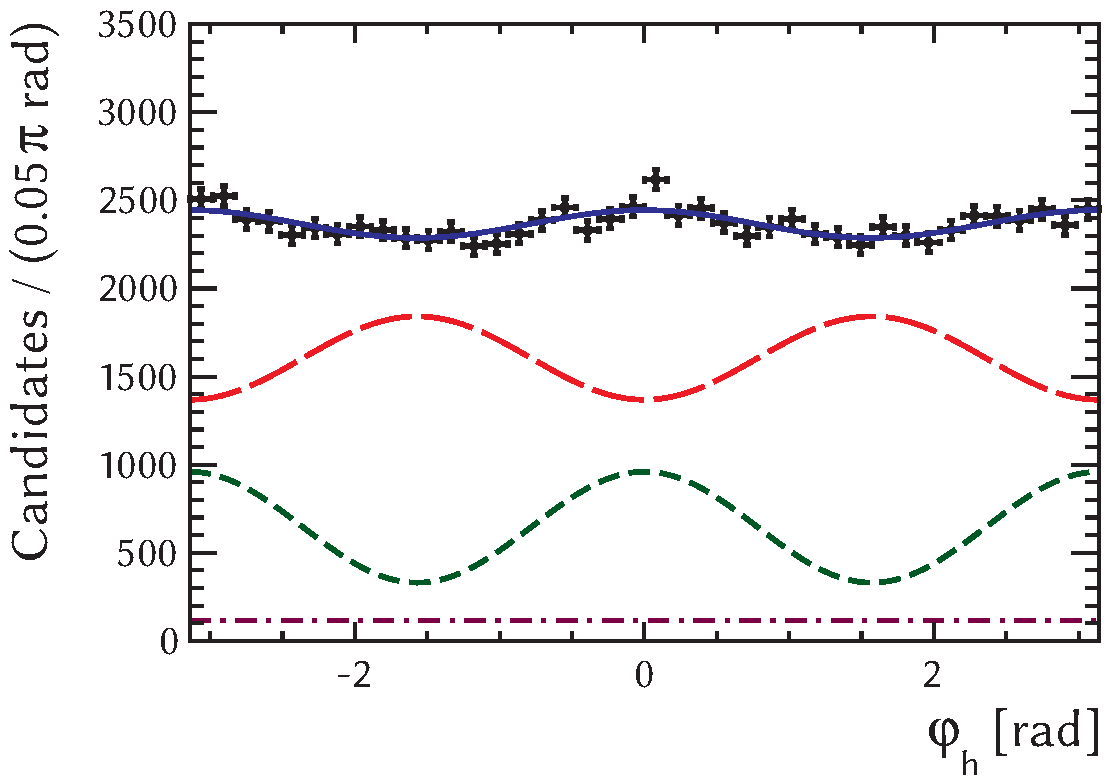
\includegraphics[width=\textwidth]{graphics/results/phi}
    \caption{}
  \end{subfigure}

  \caption{Background-subtracted distribution of decays in decay angles (data points)
           and the corresponding one-dimensional projections of the PDF (solid, blue line).
           The distributions of $\cthetaK$, $\cthetal$, and $\phihel$ are shown in Figures~(a), (b), and (c), respectively.
           Additional PDF projections are shown for the CP-even (long-dashed, red line) and CP-odd (short-dashed, green line)
           components of \BstoJpsiphi{} and for the S-wave (dashed-dotted, magenta line).}
  \label{fig:angleProjections}
\end{figure}

The solid, blue lines in Figures~\ref{fig:timeProjections} and \ref{fig:angleProjections} represent the projections of the full PDF and are
to be compared to the distributions of the data. In addition the contributions of CP-even and CP-odd intermediate states to the PDF are
shown separately. The long-dashed, red lines represent the sum of the $\magzeroSq$ and $\magparSq$ terms in the PDF, which are CP-even. The
CP-odd $\magperpSq$ and $\magSSq$ terms are shown as the short-dashed, green and dashed-dotted, magenta lines, respectively. Contributions
from interference terms are not shown. The discontinuities in the decay-time PDFs arise from statistical uncertainties in the bin
coefficients of the acceptance function.

Even though the angular dependence of the interference terms is not visible in the projection plots, they clearly show differences in the
shapes of the CP-even and CP-odd components, which enable a statistical separation. In $\cthetaK$ and $\cthetal$ the difference between
the even and odd \BstoJpsiphi{} components is made by the $\magzeroSq$ and $\magperpSq$ angular functions. Where the $\magzeroSq$ term has
a $\cos^2\theta$ behaviour, the $\magperpSq$ term has a $\sin^2\theta$ behaviour and vice versa. In $\phihel$ the $\magzeroSq$ function is
uniform, but the oscillatory behaviour for $\magparSq$ is opposite to that of the $\magperpSq$ function. The $\KK$ S-wave term is uniform
in $\cthetaK$ and $\phihel$, but proportional to $\sin^2\thetal$.

The largest contribution comes from the CP-even $\magzeroSq$ and $\magparSq$ components, which account for approximately 75\% of the
\BstoJpsiphi{} contribution. Although this cannot be seen in these projection plots, $\magparSq$ and $\magperpSq$ are roughly equal. The
S-wave accounts for approximately 5\% of the total.

From the decay-time plot with logarithmic vertical scale it is clear that the CP-even intermediate states decay faster than the CP-odd
intermediate states. Assuming small CP violation, the even states roughly correspond to the light CP eigenstate of the \BsBsbar{} system
and the odd states to the heavy CP eigenstate (Equation~\ref{eq:timeCPEvenOdd}). From this it can be inferred that the decay width of the
light eigenstate is larger and hence that $\DGs\equiv\GL-\GH$ is positive.

The plots in Figure~\ref{fig:timeProjections} show the sum of the $\Bs$ and $\Bsbar$ decay-time distributions, for which the decay-time
oscillation vanishes. Since most of the sensitivity for the CP-violation parameters comes from the amplitudes of the oscillation terms,
these projection plots contain little information on the CP-violation measurement. More information is contained in
Figure~\ref{fig:BBbarAsymmetry}, which shows the asymmetry between $\Bs$ tags and $\Bsbar$ tags.
\begin{figure}[htb]
  \centering
  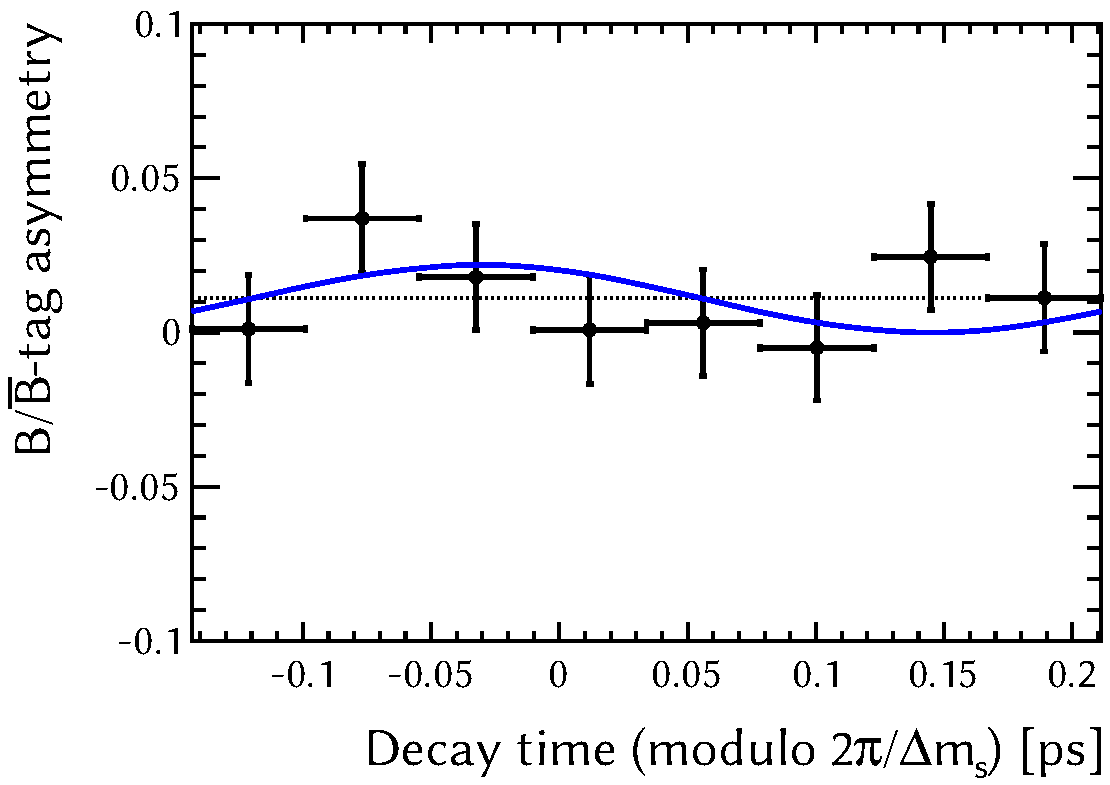
\includegraphics[width=0.75\textwidth]{graphics/results/asym}
  \caption{Background-subtracted asymmetry in the numbers of decays with $\Bs$ and $\Bsbar$ flavour tags (data points)
           and the corresponding asymmetry in the PDF (blue line) as a function of decay time.
           Data from the full decay-time range are mapped onto one period of the expected oscillation in the asymmetry.
           Decay candidates are weighted by the product of the corresponding estimated dilution factors from decay-time resolution
           and wrong tags to optimize the significance of the displayed asymmetry.}
  \label{fig:BBbarAsymmetry}
\end{figure}

The \BsBsbar-tag asymmetry is defined as
\[
  A_{\text{tag}} \equiv \frac{\#\Bs{}\text{ tags} - \#\Bsbar{}\text{ tags}}{\#\Bs{}\text{ tags} + \#\Bsbar{}\text{ tags}}
\]
and is shown in bins of decay-time for the data. This asymmetry oscillates as a function of decay time if CP symmetry is violated for
\BstoJpsiKK{} (Equations~\ref{eq:timeCPEvenOdd} and \ref{eq:timeOscill}) and if the dilution factors from flavour tagging and decay-time
resolution are nonzero. To increase the statistical significance of the displayed asymmetry all oscillation periods are projected onto the
one period of \textapprox0.35~ps that is shown in Figure~\ref{fig:BBbarAsymmetry}. The significance is further enhanced by weighting the
contribution of each decay candidate by the product of the corresponding dilution factors from tagging and resolution.

The background-subtracted asymmetry in each of the eight bins in Figure~\ref{fig:BBbarAsymmetry} is estimated by the ratio of the bin
integrals of the difference and the sum of $\Bs$-tag and $\Bsbar$-tag PDFs. The result is a mean of the asymmetry at each point in time,
weighted by a factor from the exponential decay. Because the oscillation is much faster than the decay, this weighted mean is well
approximated by the unweighted mean of the asymmetry in the PDF. The PDF asymmetry is shown in the asymmetry plot as the blue line.

Although the asymmetry plot shows an oscillation in the $\Bs$ and $\Bsbar$ PDFs, the statistical uncertainties on the data points show the
this oscillation is not significant. This indicates that that the estimates of the $\phis$ and $\Cs$ from the fit also not differ from zero
significantly. Also the overall mean \BsBsbar-tag asymmetry in the data, indicated by the dotted, black line, is not statistically
significant. A nonzero mean could arise from production and tagging asymmetries. The PDFs for $\Bs$ tags and $\Bsbar$ tags are weighted by
the number of decays in the corresponding category, which makes the mean asymmetry in the PDF equal to the value in the data by
construction.
